\subsubsection{Smarter Monte Carlo Sampling}
This project requires the understanding of the average of a function or the expected value of a random variable as an integral, knowledge of modulo arithmetic, and programming skill in Python or MATLAB.

Multivariable integrals arise in Bayesian inference, quantitative finance, and uncertainty quantification.  When the number of variables, $d$, is more than a few, the most computationally efficient methods are Monte Carlo methods, where the integral of interest is interpreted as the expectation (or population mean) of a function of a (uniform) random variable, which is then approximated by a sample mean, perhaps after a variable transformation:
\[
    \int_{[0,1]^d} f(\bx) \, \dif \bx = \Ex[f(\bX)] \approx \frac 1n \sum_{i=1}^n f(\bx_i), \qquad \text{where }\bX \sim \calu[0,1]^d.
\]

\begin{wrapfigure}{r}{0.56\textwidth}
	\centering
	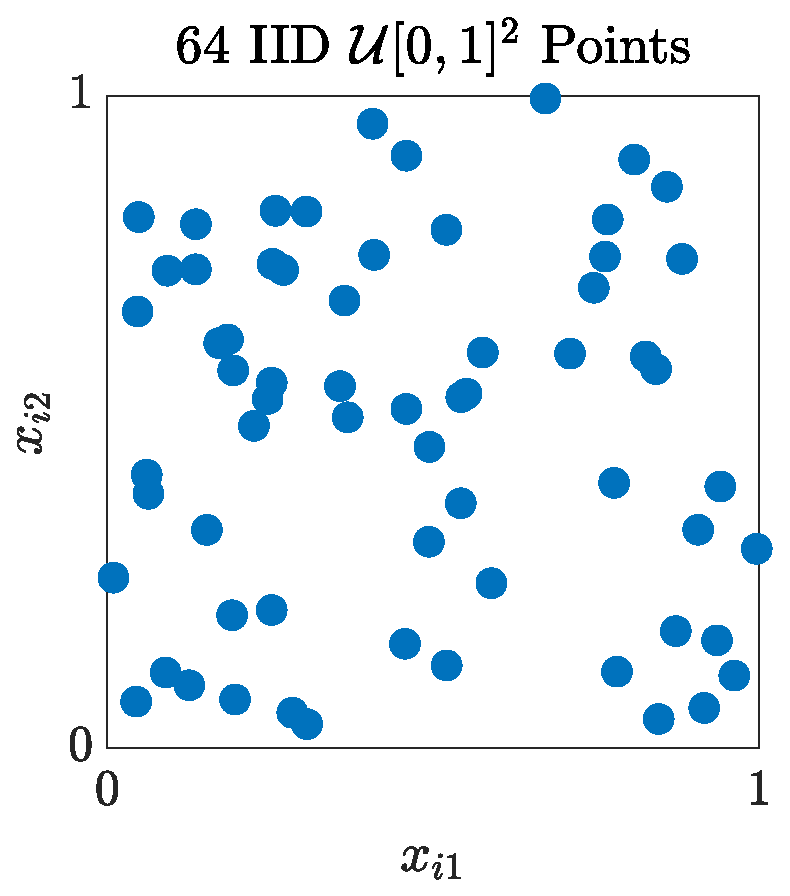
\includegraphics[height = 4.5cm]{IIDPoints.eps} \quad
	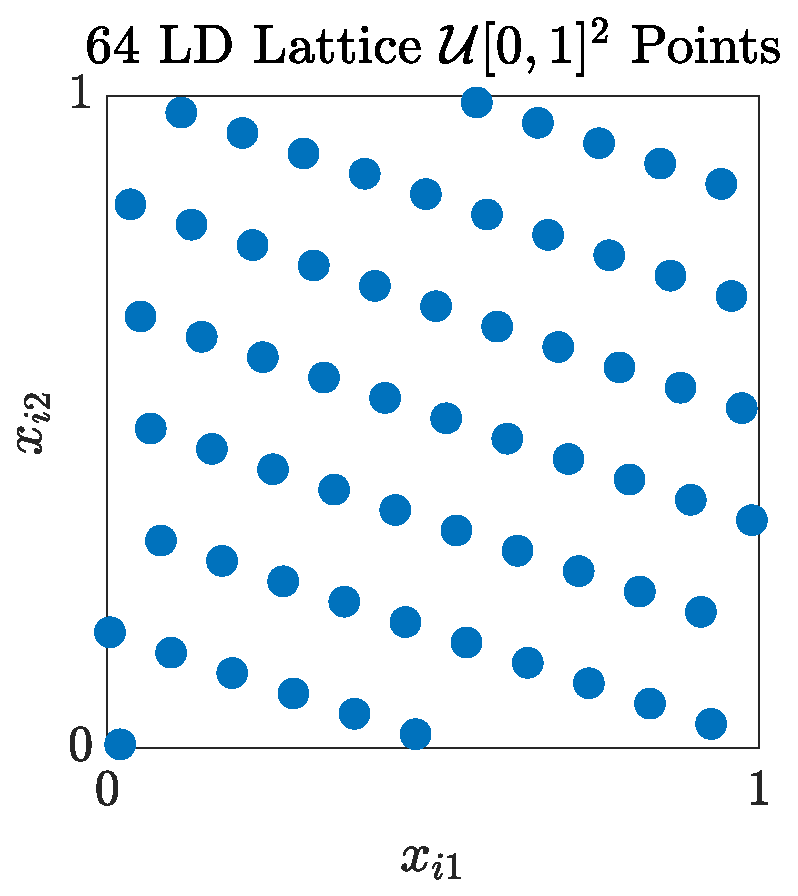
\includegraphics[height = 4.5cm]{ShiftedLatticePoints.eps}
	\caption{IID points and LD lattice points.  The LD points have fewer gaps and clusters of points than the IID points. \label{fig:iid_vs_ld}}
\end{wrapfigure}
The number of function values, $n$, required to meet an absolute error tolerance of $\varepsilon$ using independent and identically distributed (IID) $\bx_i$ is $\Order(\varepsilon^{-2})$, but this cost decreases significantly to $\Order(\varepsilon^{-1+\delta})$ when using low discrepancy (LD) $\bx_i$, as depicted in Fig.\ \ref{fig:iid_vs_ld}.  LD sequences give faster convergence because they are more evenly distributed on $[0,1]^d$.
Choi, Ding, Hickernell, and collaborators have developed the GAIL MATLAB library \cite{ChoEtal21a,TonEtAl22a} and the QMCPy Python library \cite{ChoEtal22a,QMCPy2020a}, which implement IID and LD methods for approximating multivariate integrals to specified error tolerances \cite{HicEtal14a,HicJim16a,JimHic16a,HicEtal17a,RatHic19a,JagHic22a}.  

The specific {\bf learning goals} for students are the following:
\begin{itemize}[leftmargin=.5cm]
    \item Explain the relationship between average and integral for multidimensional problems;
    \item Compare the performance of different Monte Carlo algorithms; and
    \item Use one or more software libraries to perform numerical experiments to solve  complex problems;
    \item Contribute to software packages.
\end{itemize}
The specific {\bf research goals} for students are one of the following:
\begin{itemize}[leftmargin=.5cm]
\item Identify importance sampling methods---or equivalently variable transformations---that smooth peaky integrands, such as those arising in Bayesian inference;

\item Measure the efficacy of the median-of-means estimators recently proposed by Pan and Owen using randomized digital sequences \cite{SPAMOM22} and Goda and L'Ecuyer using  lattice sequences
\cite{CFMQMC}; these simple generators converge faster than expected, but we do not have stopping rules for them, and they have only been tried on a limited number of examples; and 

\item Demonstrate via well chosen examples how QMCPy or GAIL can be integrated with other popular libraries, such as FEniCS \cite{AlnaesEtal2015,LoggEtal_11_2012}, Dakota \cite{DakotaUsersManual} and MUQ \cite{MUQ} for solving (partial) differential equations with random coefficients and other problems in uncertainty quantification.
\end{itemize}